\section{Diseño Metodológico}

El desarrollo de este trabajo se divide en dos semestres, con una duración total de un año, y se estructura en fases progresivas que permiten alcanzar tanto el objetivo general como los objetivos específicos planteados.

\subsection*{Primer Semestre}

El primer semestre estará dedicado a la \textbf{formulación y preparación del modelo físico}, junto con la \textbf{implementación computacional} necesaria para ejecutar simulaciones en el marco de la Magnetohidrodinámica  \sout{Resistiva Relativista}  \ser{Relativista Resistiva} (RRMHD). Esta etapa incluye la revisión de las ecuaciones fundamentales del modelo, la definición de condiciones iniciales (como el perfil de velocidad, la orientación del campo magnético y los valores de resistividad) y la validación del solucionador numérico disponible. Estas actividades permitirán cumplir el \textbf{primer objetivo específico}: \textbf{analizar el efecto de la resistividad en la tasa de crecimiento lineal y lograr simular el crecimiento no lineal de las inestabilidades}.

De forma paralela, se desarrollarán scripts automatizados para ejecutar simulaciones con distintas configuraciones, y se realizarán pruebas con tiempos de integración reducidos para verificar la estabilidad numérica y la consistencia física del sistema.

\subsection*{Segundo Semestre}

Durante el \textbf{segundo semestre}, el enfoque se centrará en la \textbf{ejecución extensiva de simulaciones} y en el \textbf{análisis cuantitativo de los resultados}. Se explorarán variaciones sistemáticas en la resistividad y en la orientación del campo magnético, con el objetivo de estudiar su influencia en la evolución de las inestabilidades. Estas simulaciones de mayor duración permitirán observar la transición desde el régimen lineal hasta fases no lineales, incluyendo la formación de vorticidad y estructuras turbulentas. Esto contribuirá al cumplimiento de los \textbf{objetivos específicos 2, 3 y 4}.

En concreto, Se \textbf{analizará la influencia de la resistividad en la generación y evolución de estructuras secundarias}, como vórtices, en la interfaz de corte (Objetivo 2).
Se \textbf{investigará el impacto de la difusión magnética en la evolución espacio-temporal de variables globales}, como el campo magnético, el campo eléctrico y el campo de velocidades en la malla de simulación (Objetivo 3).
Y por ultimo Se \textbf{evaluará el papel de la orientación y la intensidad del campo magnético en la estabilización o amplificación de las perturbaciones} en la interfaz de corte (Objetivo 4).

Para cada conjunto de simulaciones, se extraerán variables globales como energía cinética, presión total, vorticidad y la evolución temporal de las perturbaciones en la interfaz. Estos datos permitirán cuantificar la tasa de crecimiento de la inestabilidad, detectar patrones recurrentes y validar las hipótesis propuestas. Finalmente, los resultados se sistematizarán en reportes gráficos y escritos, útiles tanto para la redacción del informe final del trabajo de grado como para la elaboración de presentaciones tipo póster o exposiciones orales.

Esta organización anterior, se condensa en la siguiente tabla: \ser{(en la tabla hace falta colocar un tiempo para la escritura y revisión de la tesis, minimo dos meses)}

\begin{figure}[h]
    \centering
    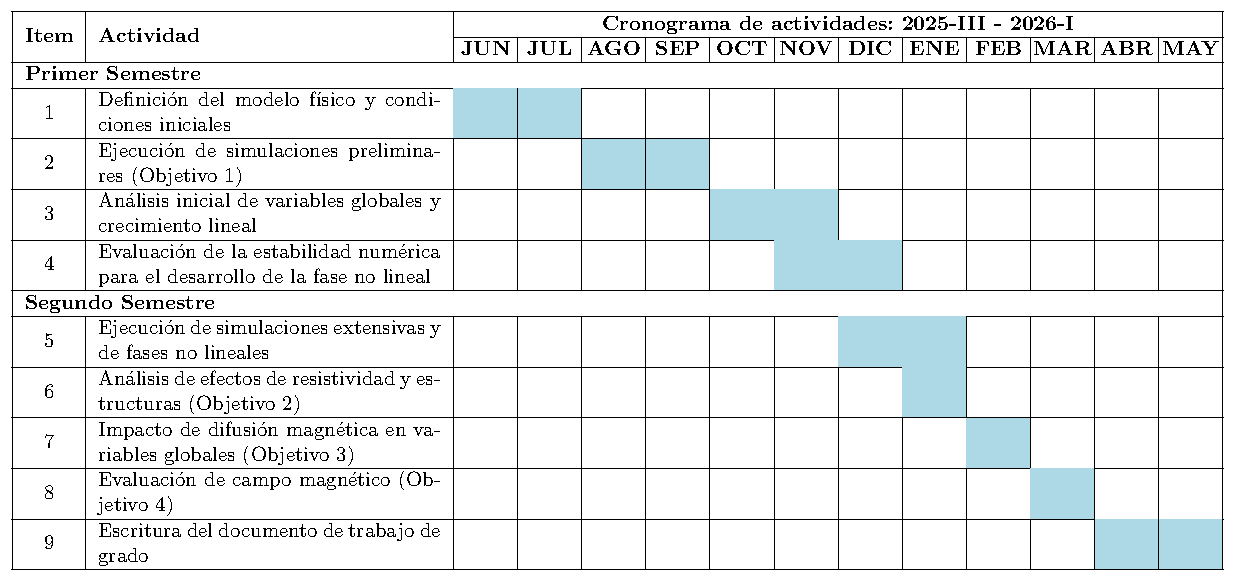
\includegraphics[width=0.9\textwidth]{source/image/tabla.pdf}
    \caption{Fases del proyecto}
    \label{fig:tabla}
\end{figure}
